\documentclass{beamer}
\title[JVMTIPROF]{JVMTIPROF: An extension to the Java Virtual Machine Tool Infrastructure for building profiling agents}
\author{Denilson das Mercês Amorim}
\institute[UFBA]{Universidade Federal da Bahia}
\date{2022}

\usepackage{listings} 
\lstset{basicstyle = \ttfamily}
\definecolor{patchadd}{rgb}{0.0, 0.65, 0.31}

\usetheme{Madrid}

%\usepackage{pgfpages}
%\setbeamertemplate{note page}[plain]
%\setbeameroption{show notes on second screen=right}

\logo{
\includegraphics[height=1cm]{ufba.pdf}}

% Insert a slide at every \section definition.
\AtBeginSection{
    \frame{
        \begin{center}
        \usebeamerfont*{frametitle}
        \insertsection
        \end{center}
    }
}

\begin{document}

\frame{\titlepage}

\begin{frame}
\frametitle{Table of Contents}
\tableofcontents
\end{frame}

\section{Introduction}

\begin{frame}
\frametitle{Motivation}
\begin{itemize}
\item<1-> Profiling commonly used to identify application bottlenecks.
\item<1-> Instrumentation fundamental part of profiling infrastructure.
\item<1-> Tool-building systems can be used to build profilers.
\item<1-> JVMTI exists in the Java ecosystem but is too bare-bones.
\note{Instrumenting method entry and exit efficiently requires direct class file and bytecode manipulation!}
\end{itemize}
\end{frame}

\begin{frame}
\frametitle{Contribution}
\begin{itemize}
\item<1-> JVMTIPROF
\begin{itemize}
\item An extension to JVMTI with high-level functionality.
\item Same patterns, idioms and types -- reduced learning curve.
\item Agent developers can focus more on methods than infrastructure.
\end{itemize}
\item<2-> How to extend JVMTI without source-level modifications.
\end{itemize}
\end{frame}

\section{Background}

\begin{frame}
\frametitle{Instrumentation}
\begin{itemize}
\item Technique to add auxiliary code to existing programs.
\item Can be \emph{static} (i.e. compile-time) or \emph{dynamic} (i.e. runtime).
\item \emph{Function hooking} is the act of instrumenting function boundaries.
\item Profiling, program analysis, code coverage, just-in-time compilation...
\end{itemize}
\end{frame}

\begin{frame}
\frametitle{Profiling}
\begin{itemize}
\item Dynamic program analysis to measure performance.
\item Typically used to identify hot paths.
\item Classified in \emph{sampling profilers} and \emph{instrumenting profilers}.
\item Can feed profiled-guided optimization algorithms.
\note{Case study: Profile-guided optimizing compilers.}
\end{itemize}
\end{frame}

\begin{frame}
\frametitle{Sampling in Unix-like Systems}
\begin{itemize}
\item Sampling profilers need to sample the call stack trace.
\item Application-wide timer -- \lstinline{ITIMER_PROF}.
\item Notification through signals -- \lstinline{SIGPROF}.
\item Handler must be \emph{async-signal-safe}.
\note{Example: Deadlock if they try to hold same lock as interrupted thread.}
\note{Primitive memory-operations and subset of system calls.}
\end{itemize}
\end{frame}

\begin{frame}
\frametitle{Java Virtual Machine}
\begin{itemize}
\item Abstract Machine.
\note{Exists as an specification}
\item Executes code independently of hardware and operating system.
\item Has its own instruction-set.
\item Several concrete implementations (hardware or software-based).
\item Oracle's HotSpot is the reference implementation.
\end{itemize}
\end{frame}

\begin{frame}
\frametitle{Java Virtual Machine}
\begin{itemize}
\item Several programming languages targeting the JVM.
\item Java, Scala, Clojure, JRuby, Jython...
\item Widely popular in the software industry.
\item Garbage-collected memory management.
\end{itemize}
\end{frame}

\begin{frame}
\frametitle{Java Virtual Machine -- Execution Pipeline}
\begin{itemize}
\item A program compiles into a set of class files.
\item A \emph{class file} contains JVM instructions (\emph{bytecode}).
\item Class files are loaded and linked by the \emph{class loader}.
\item JVM interprets the class bytecode once loaded.
\end{itemize}
\end{frame}

\begin{frame}
\frametitle{Java Virtual Machine -- JIT Compiler}
\begin{itemize}
\item Interpretation is slow!
\item Just-in-time compilation to the rescue.
\item Bytecode is compiled to machine code on-the-fly.
\item JIT performs profile-guided compiler optimizations.
\note[itemize]{
    \item Tiered-compilation.
    \item Four levels of compilation.
    \item Optimizes and deoptimizes.
    \item Profile built from instrumentation of loop-backedges and method calls.
}
\end{itemize}
\end{frame}

\begin{frame}
\frametitle{Java Native Interface (JNI)}
\begin{itemize}
\item API for bytecode to interoperate with native code.
\item Can invoke C++ functions from Java and vice-versa.
\item Per-thread \emph{JNI environment} -- function-table and state.
\end{itemize}
\end{frame}

\begin{frame}
\frametitle{Java Native Interface (JNI)}
\begin{figure}[b]
\par\noindent\begin{minipage}[t]{.45\textwidth}
\lstinputlisting[language=Java,frame=tlrb,basicstyle=\small]{src/listing/JNIExample.java}
\end{minipage}\hfill
\begin{minipage}[t]{.52\textwidth}
\lstinputlisting[language=C++,frame=tlrb,basicstyle=\small]{src/listing/JNIExample.cpp}
\end{minipage}
\end{figure}
\end{frame}

\begin{frame}
\frametitle{Java Native Interface (JNI)}
\centering
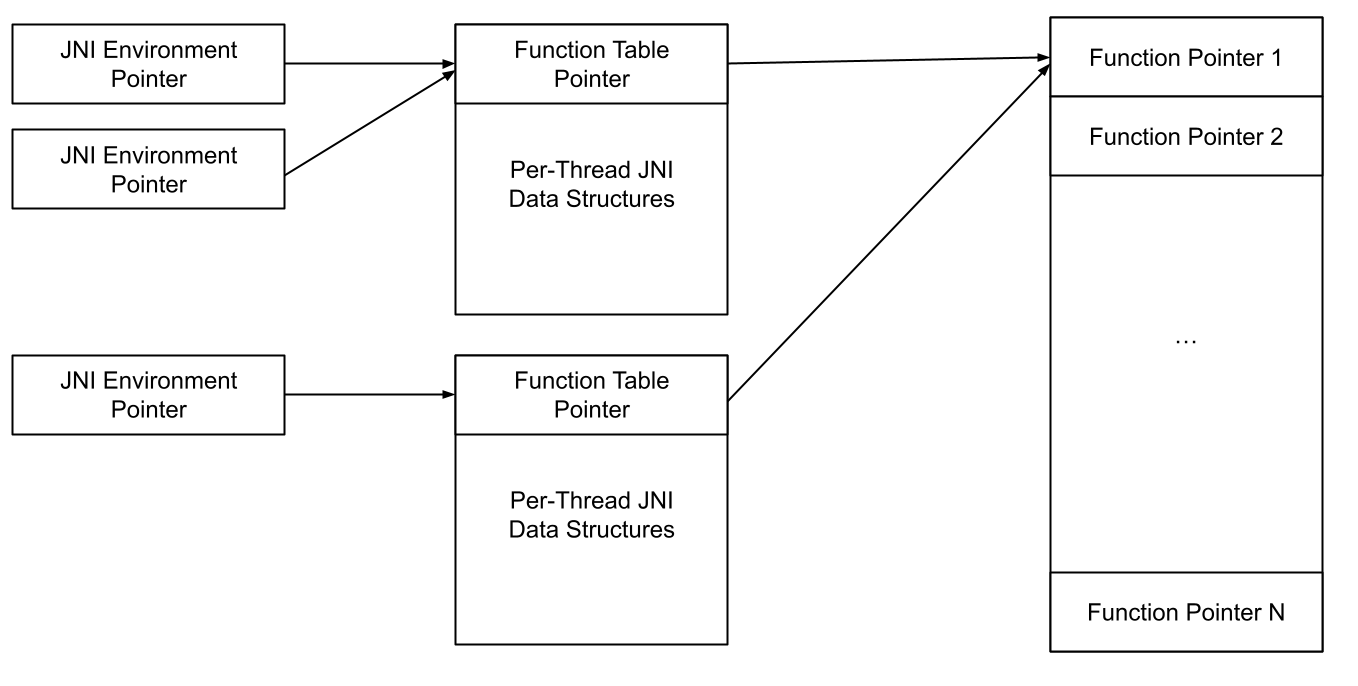
\includegraphics[width=0.81\textwidth]{src/figure/jni_function_table.png}
\end{frame}

\begin{frame}
\frametitle{JVM Tool Interface (JVMTI)}
\begin{itemize}
\item API for native agents to build development and monitoring tools.
\item Can inspect VM states and react to events.
\item Same approach as JNI (data types, function-table, etc).
\item Pay only for what you need attitude.
\end{itemize}
\end{frame}

\begin{frame}
\frametitle{JVM Tool Interface (JVMTI)}
\lstinputlisting[language=C++,frame=tb,basicstyle=\tiny]{src/listing/example-jvmti.slide.cpp}
\end{frame}

\begin{frame}
\frametitle{Java Virtual Machine -- Safepoints}
\begin{itemize}
\item Point of execution in which all root object references are known.
\item Used to implement garbage collection, thread dumps, etc.
\item Program is in a safepoint only at specific points of JIT-compiled code.
\end{itemize}
\end{frame}

\begin{frame}
\frametitle{Java Virtual Machine -- Safepoint Polls}
\begin{itemize}
\item JIT-compiled code can only know root of objects through GC maps.
\item GC maps contain stack frame locations the objects are stored.
\item Memory intensive -- cannot generate for every machine instruction.
\item Maps created only for specific instructions -- the \emph{safepoint polls}.
\item Method entry/exit and loop backedges.
\end{itemize}
\end{frame}

\begin{frame}
\frametitle{Java Virtual Machine -- Time to Safepoint}
\begin{itemize}
\item Certain operations must bring all threads to a safepoint.
\item It takes a little while -- known as \emph{time to safepoint}.
\item Blocks safepointed threads, performs operation, resumes threads.
\item A bit expensive.
\end{itemize}
\end{frame}

\begin{frame}
\frametitle{Java Virtual Machine -- Safepoint Bias}
\begin{itemize}
\item JVMTI provides \lstinline{GetStackTrace} et al.
\item Requires thread to be in a safepoint!
\item Thus can only sample safepoint locations -- \emph{safepoint bias}.
\item Additional interference of time to safepoint.
\end{itemize}
\end{frame}

\begin{frame}
\frametitle{Java Virtual Machine -- Safepoint Bias}
\begin{itemize}
\item Non-biased profilers exist e.g. \lstinline{honest-profiler}.
\item Requires an undocumented HotSpot API -- \lstinline{AsyncGetCallTrace}.
\item Cannot trace kernel and native code.
\item ...but \lstinline{perf} hybrids can e.g. \lstinline{async-profiler}.
\end{itemize}
\end{frame}

\begin{frame}
\frametitle{Elasticsearch}
\begin{itemize}
\item Distributed search engine written in Java.
\item Provides indexing and querying interfaces.
\end{itemize}
\end{frame}

\begin{frame}
\frametitle{Dynamic Frequency Scaling (DFS)}
\begin{itemize}
\item Technique for improving power efficiency on multi-core systems.
\item Adjusts processor frequency according to application's demand.
\item Linux implements DFS on its \emph{Ondemand} governor.
\end{itemize}
\end{frame}

\begin{frame}
\frametitle{Related Work}
\begin{itemize}
\item Static Instrumentation
\begin{itemize}
\item BCEL (DAHM, 1999)
\item ASM (BRUNETON et al., 2002)
\item Javassist (CHIBA; NISHIZAWA, 2003)
\item SOOT (VALLéE-RAI et al., 2010)
\end{itemize}
\item Dynamic Instrumentation
\begin{itemize}
\item FERRARI (BINDER et al., 2007)
\note{FERRARI statically instruments core classes and an Java agent for the others}
\item DiSL (MAREK et al., 2012)
\note{DiSL forwards classes from a JVMTI agent to a bootstrapped VM.}
\end{itemize}
\item All of them are written in and for use within Java boundaries.
\end{itemize}
\end{frame}

\begin{frame}
\frametitle{Related Work}
\begin{itemize}
\item JNIF (MASTRANGELO; HAUSWIRTH, 2014)
\begin{itemize}
\item Java Native Instrumentation Framework
\item Static instrumentation in native code.
\item Can be used from JVMTI's hooks to perform dynamic instrumentation.
\end{itemize}
\item Our work is the the first fully native dynamic instrumentation framework for Java (as far as we know).
\end{itemize}
\end{frame}


\section{Methodology}

\begin{frame}
\frametitle{Design}
\begin{itemize}
\item Similar to JVMTI -- just like it is similar to JNI.
\item Environment created with \lstinline{jvmtiProf_Create}.
\item Can perform efficient \emph{method interception}.
\item Can perform asynchronous \emph{call stack tracing}.
\item Can perform execution sampling.
\item Pay only for what you ask for ;)
\end{itemize}
\end{frame}

\begin{frame}
\frametitle{Example -- Sample and Print Call Stack}
\lstinputlisting[language=C++,frame=t,basicstyle=\tiny]{src/listing/demo-sample-execution.slide1.cpp}
\end{frame}

\begin{frame}
\frametitle{Example -- Sample and Print Call Stack}
\lstinputlisting[language=C++,frame=b,basicstyle=\tiny]{src/listing/demo-sample-execution.slide2.cpp}
\end{frame}

\begin{frame}
\frametitle{Implementation}
\begin{itemize}
\item Uses some events from JVMTI to implement its functionalities.
\item Collision between JVMTIPROF and JVMTI's API client desires.
\item Solution: Redirect JVMTI function-table to JVMTIPROF managed functions.
\end{itemize}
\end{frame}

\begin{frame}
\frametitle{Method Interception}
\begin{itemize}
\item Achieved by instrumenting class bytecode.
\item JVMTI's \lstinline{ClassFileLoadHook} used for intercepting class loading.
\item Intercepted method invokes JVMTIPROF which invokes API client.
\end{itemize}
\end{frame}

\begin{frame}[fragile]
\frametitle{Method Interception}
\centering
\lstinline{SetMethodEventFlag("Example", "sum", "(II)I");}
\medskip
\begin{lstlisting}[language=Java,frame=tbrl,escapechar=@,basicstyle=\tiny,xleftmargin=0.2\textwidth,xrightmargin=0.2\textwidth]
@\color{patchadd}public class JVMTIPROF \{@
    @\color{patchadd}public static native void onMethodEntry(long hookPtr);@
    @\color{patchadd}public static native void onMethodExit(long hookPtr);@
@\color{patchadd}\}@

public class Example {

    @\color{patchadd}static final long sumHookPtr = /* determined at runtime */;@

    public int sum(int a, int b) {
        @\color{patchadd}JVMTIPROF.onMethodEntry(sumHookPtr);@
        @\color{patchadd}try \{@
            return a + b;
        @\color{patchadd}\} finally \{@
            @\color{patchadd}JVMTIPROF.onMethodExit(sumHookPtr);@
        @\color{patchadd}\}@
    }
}
\end{lstlisting}
\end{frame}

\begin{frame}
\frametitle{Execution Sampling}
\begin{itemize}
\item Just like explained in \emph{Sampling in Unix-like Systems}.
\item \lstinline{CLOCK_PROCESS_CPUTIME_ID} and \lstinline{SIGPROF}.
\item Interval set by \lstinline{SetExecutionSamplingInterval}.
\item Callback must be async-signal-safe.
\item Callback must consume little CPU time -- blocking a VM thread.
\note{Usually handler uses async-signal-safe data structure and process in another thread.}
\end{itemize}
\end{frame}

\begin{frame}
\frametitle{Call Stack Trace}
\begin{itemize}
\item \lstinline{GetStackTraceAsync} -- interface similar to JVMTI.
\item Implemented by means of HotSpot's \lstinline{AsyncGetCallTrace}.
\item Async-signal-safe.
\item Does not require a safepoint -- bias free.
\item We force the VM to generate GC maps at non-safepoints.
\end{itemize}
\end{frame}

\section{Evaluation}

\begin{frame}
\frametitle{Evaluation}
\begin{itemize}
\item Profile-guided Frequency Scaling for Latency-Critical Search Workloads (MEDEIROS et al., 2021)
\begin{itemize}
\note{a.k.a. Hurryup}
\item Instruments Elasticsearch's hot functions with enter/exit events.
\item Uses these events to adapt processor core frequencies.
\item Saves energy while meeting response deadline. % compared to Ondemand
\item Uses JVMTI for the job!
\end{itemize}
\item What if we replace JVMTI with JVMTIPROF?
\end{itemize}
\end{frame}

\begin{frame}
\frametitle{Experimental Setup}
\begin{itemize}
\item Bare-metal server provided by Chameleon Cloud
\begin{itemize}
\item Intel Xeon Gold 6126 (Skylake)
\item 196GB of DRAM
\item 220GB of SSD
\end{itemize}
\item Ubuntu 20.04 (Linux kernel 5.4)
\item Elasticsearch 6.5.4
\item OpenJDK 8u342
\end{itemize}
\end{frame}

\begin{frame}
\frametitle{Experimental Setup}
\begin{itemize}
\item<1-> 24 physical cores, two-socket CPU.
\begin{itemize}
\item One socket for Elasticsearch.
\item Another for load-generator (FABAN).
\item Hyper-threading turned off.
\end{itemize}
\item<2-> Wikipedia indexed in Elasticsearch.
\item<3-> Intel RAPL used for energy measurements.
\item<4-> Load-generation runs for 20 minutes, six times.
\begin{itemize}
\item Each client issues one request per second.
\item Low Load: 4 clients.
\item High Load: 12 clients.
\end{itemize}
\item<5-> Report mean and standard deviation for 99-percentile latency and energy consumption.
\end{itemize}
\end{frame}

\begin{frame}
\frametitle{Baseline}
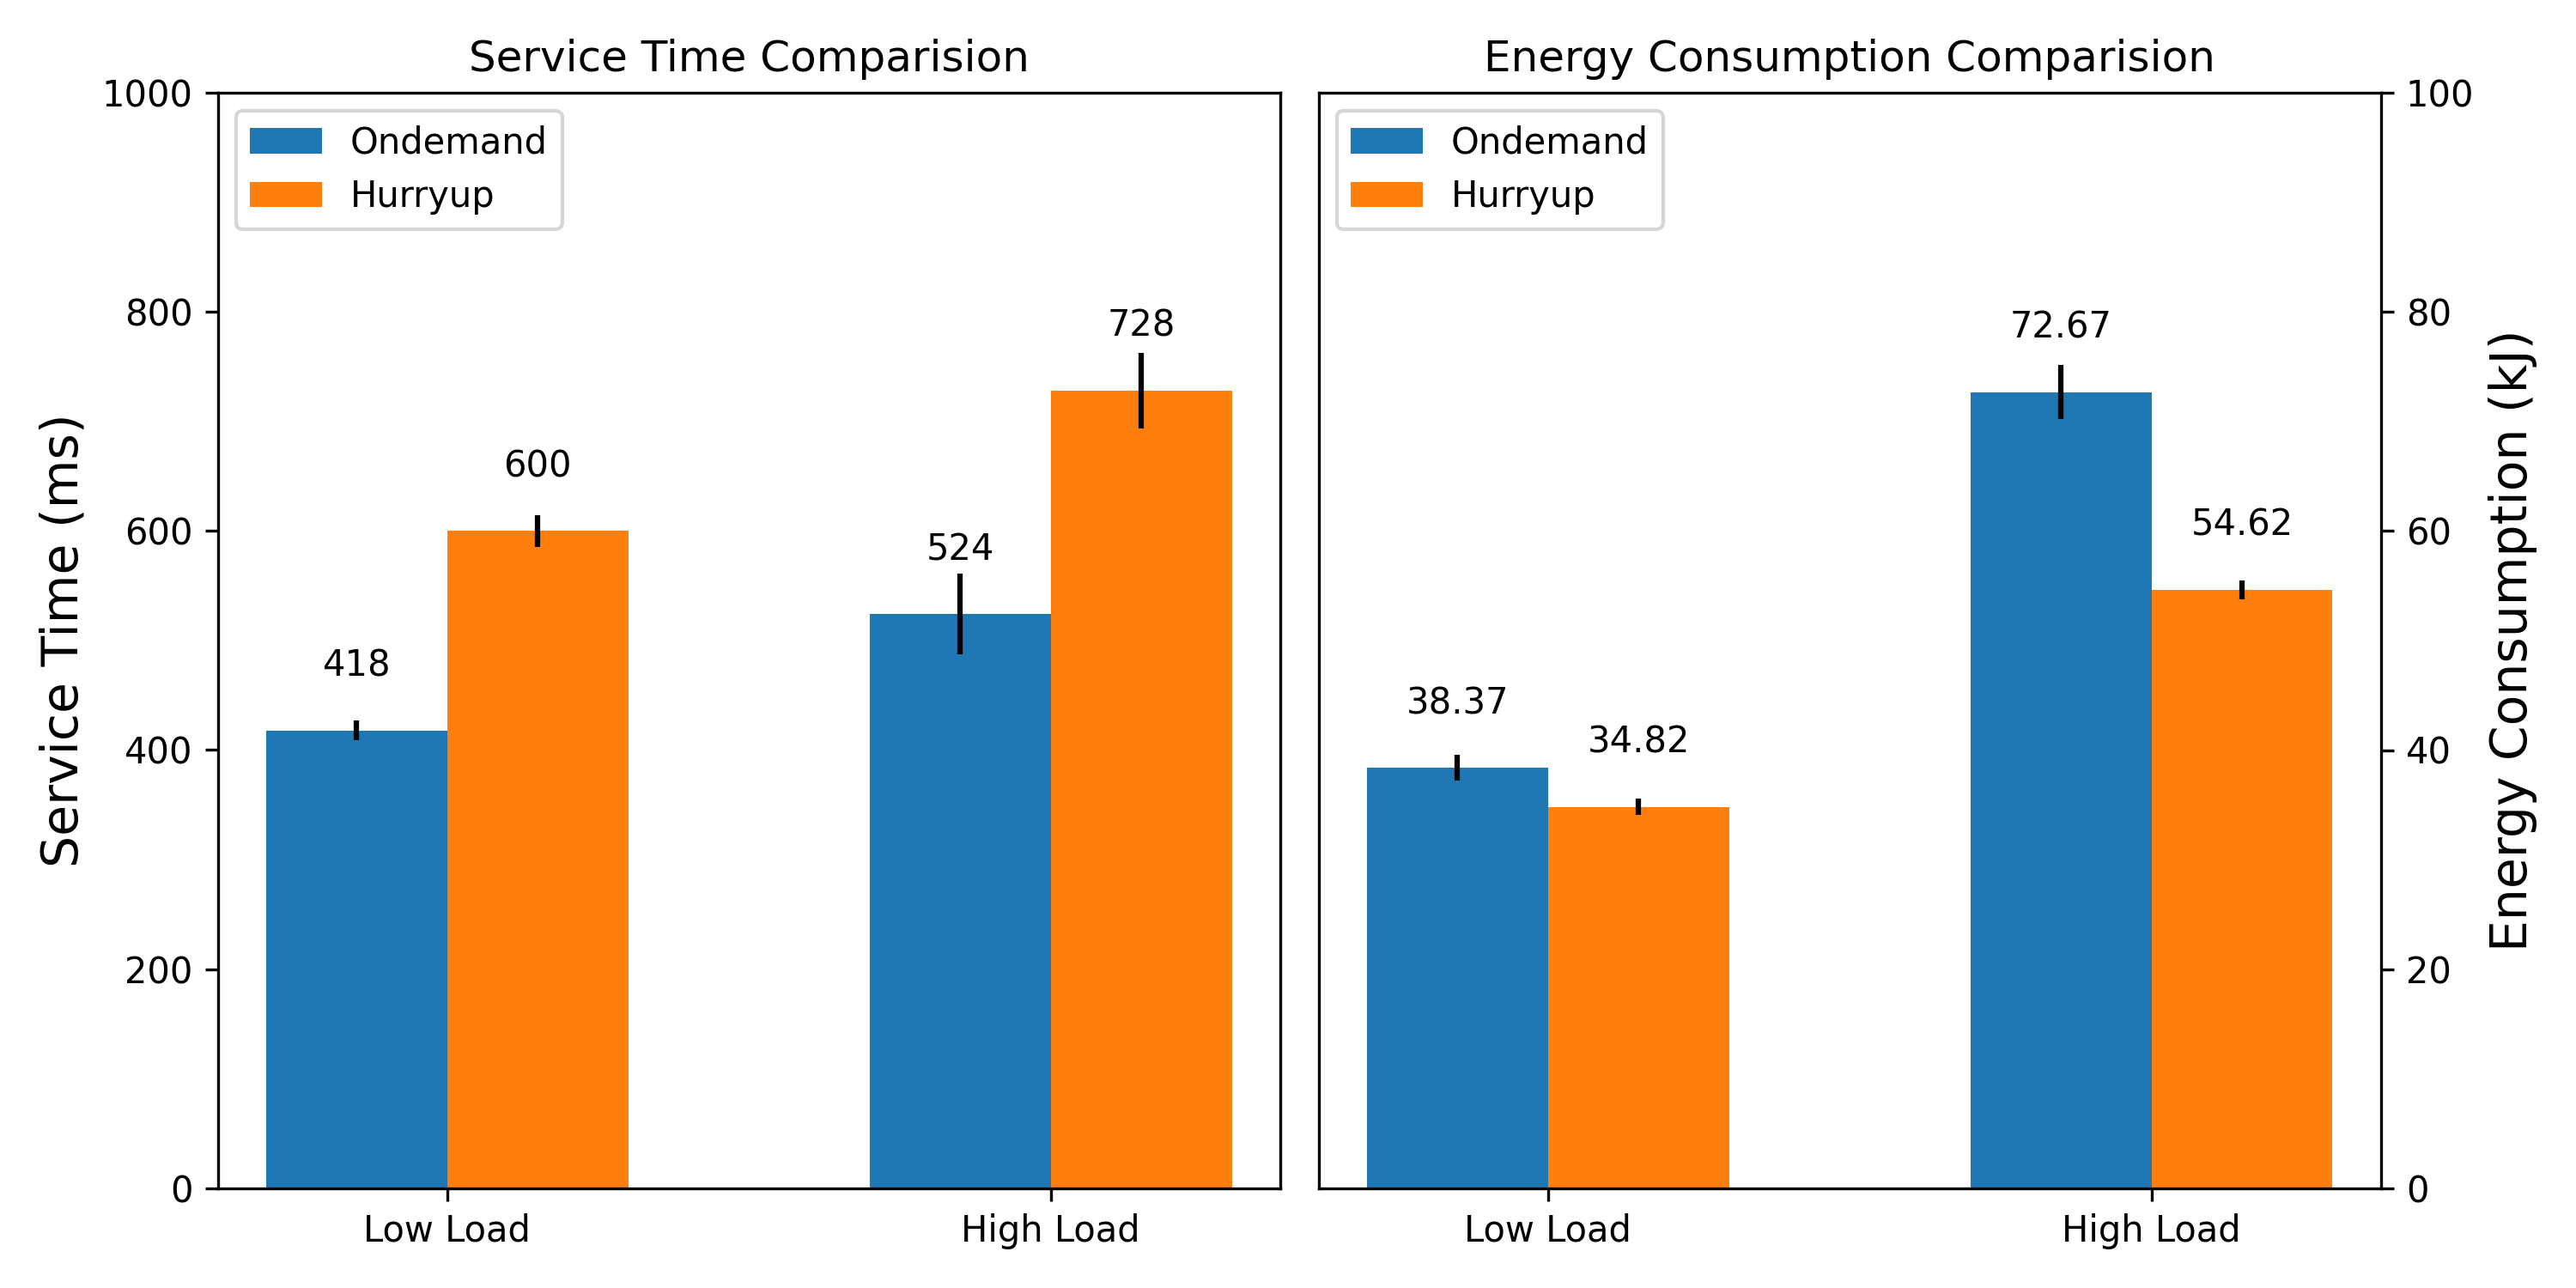
\includegraphics[width=1.0\textwidth]{src/figure/ondem_vs_hup.png}
\note{Hurryup saves up to 25\% in energy compared to Ondemand}
\end{frame}

\begin{frame}
\frametitle{Results}
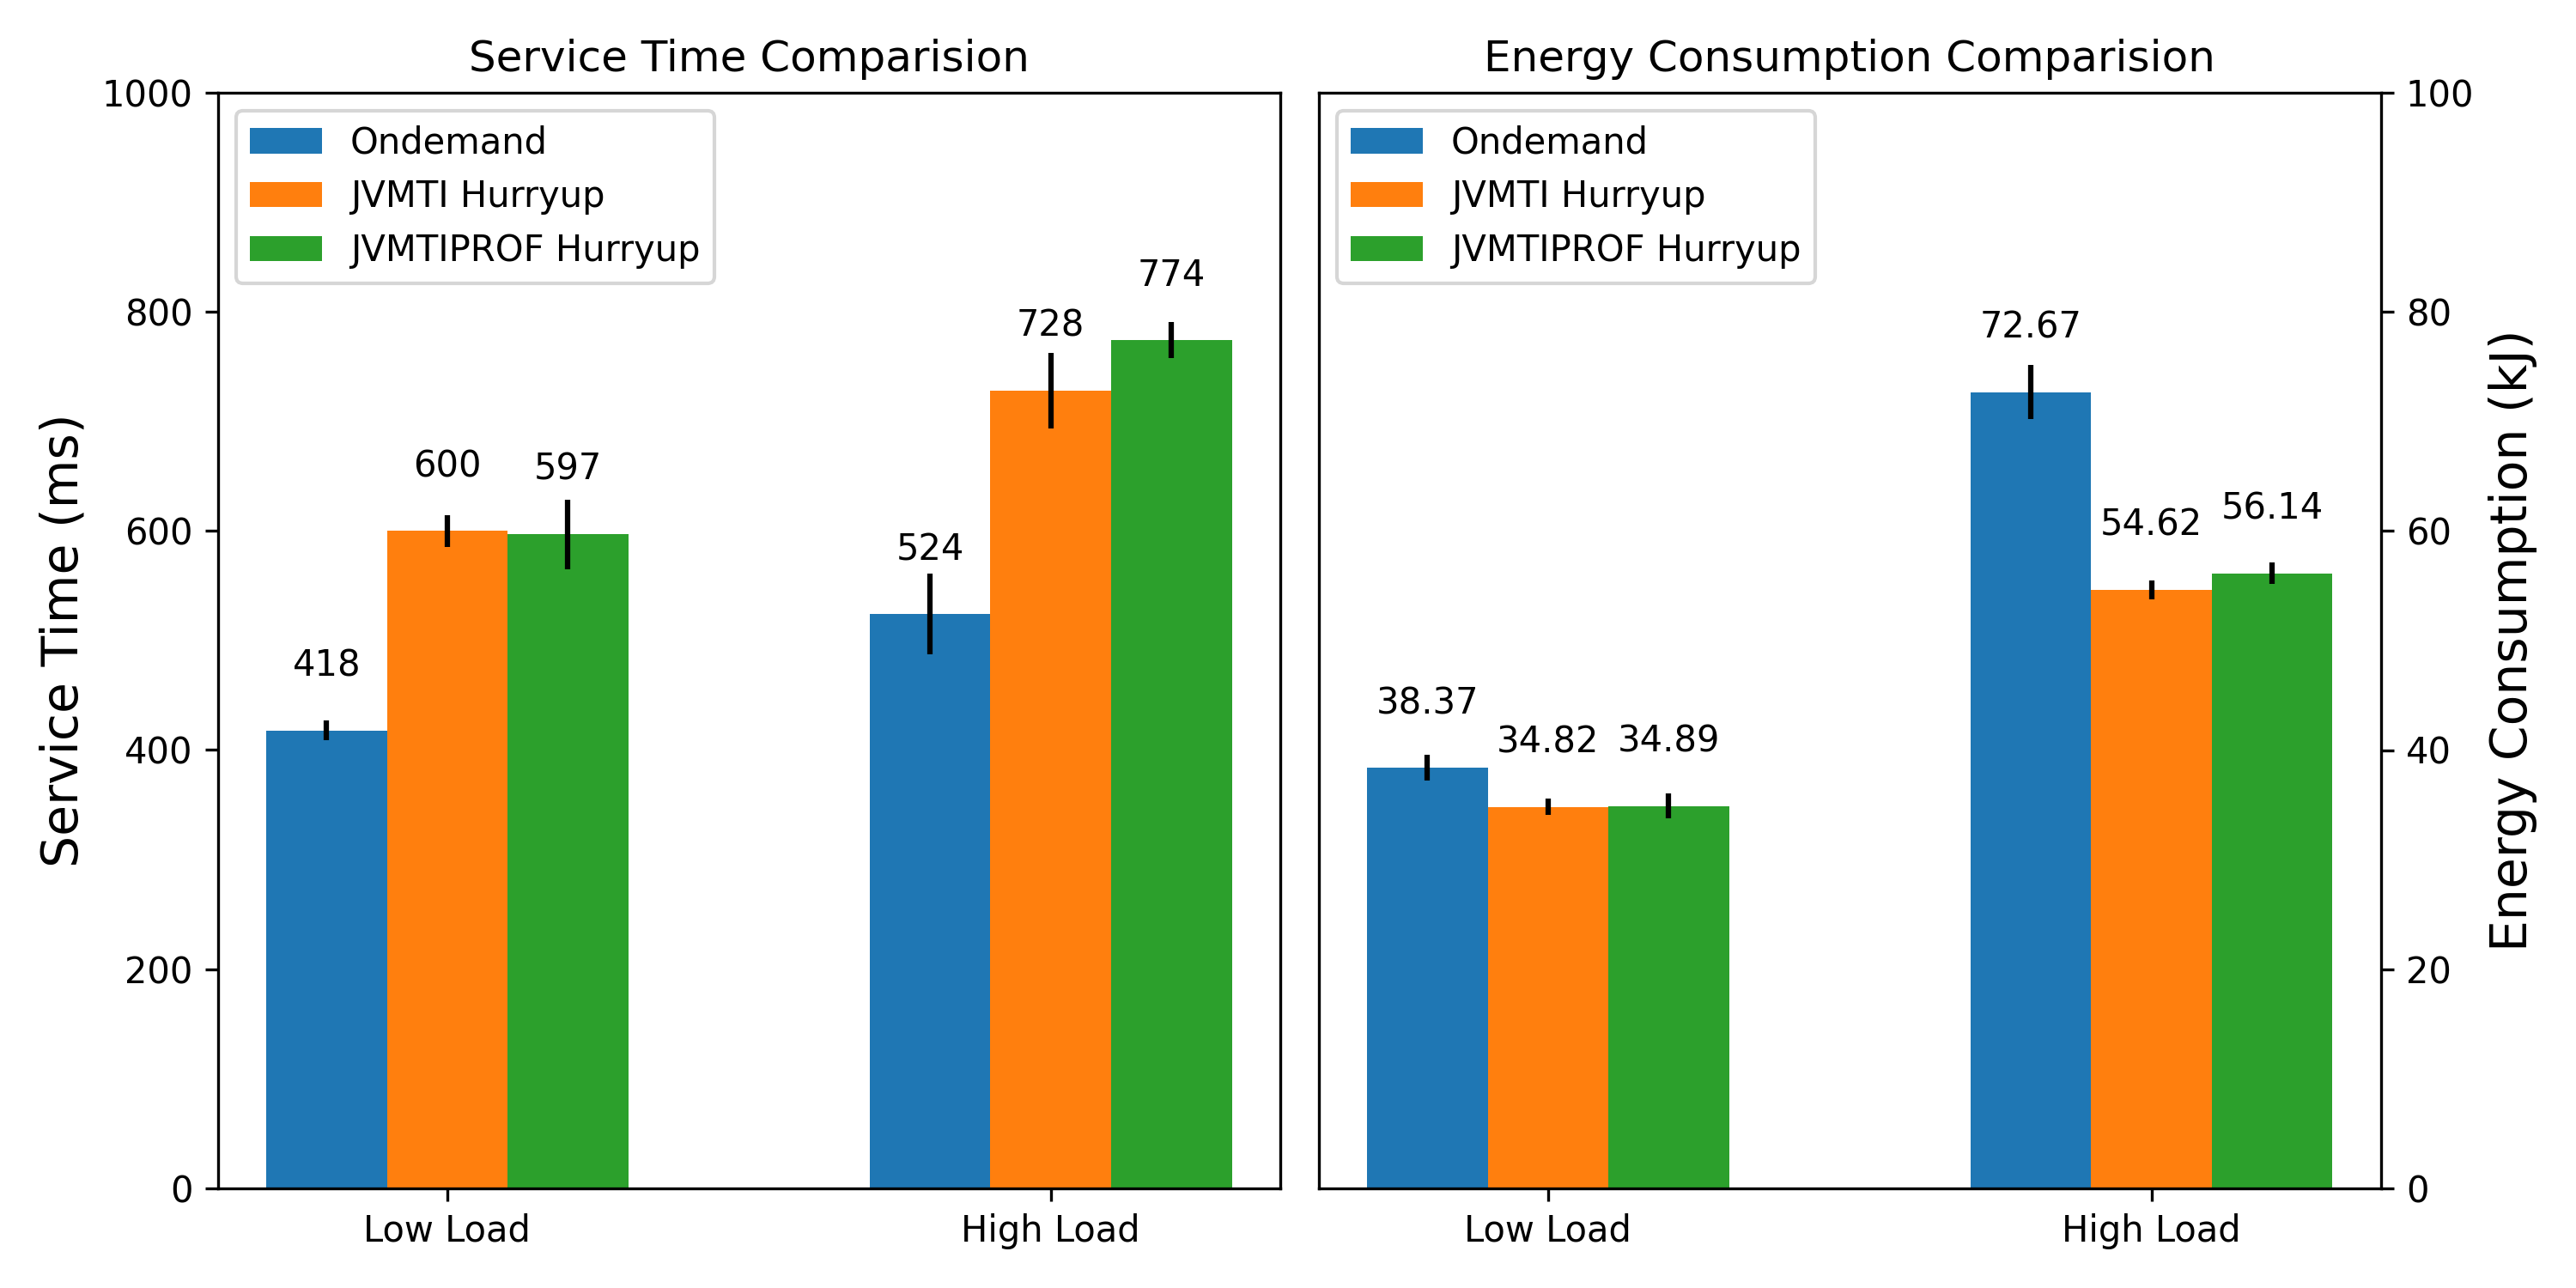
\includegraphics[width=1.0\textwidth]{src/figure/ondem_vs_hup_vs_newhup.png}
\end{frame}

\begin{frame}
\frametitle{Overhead}
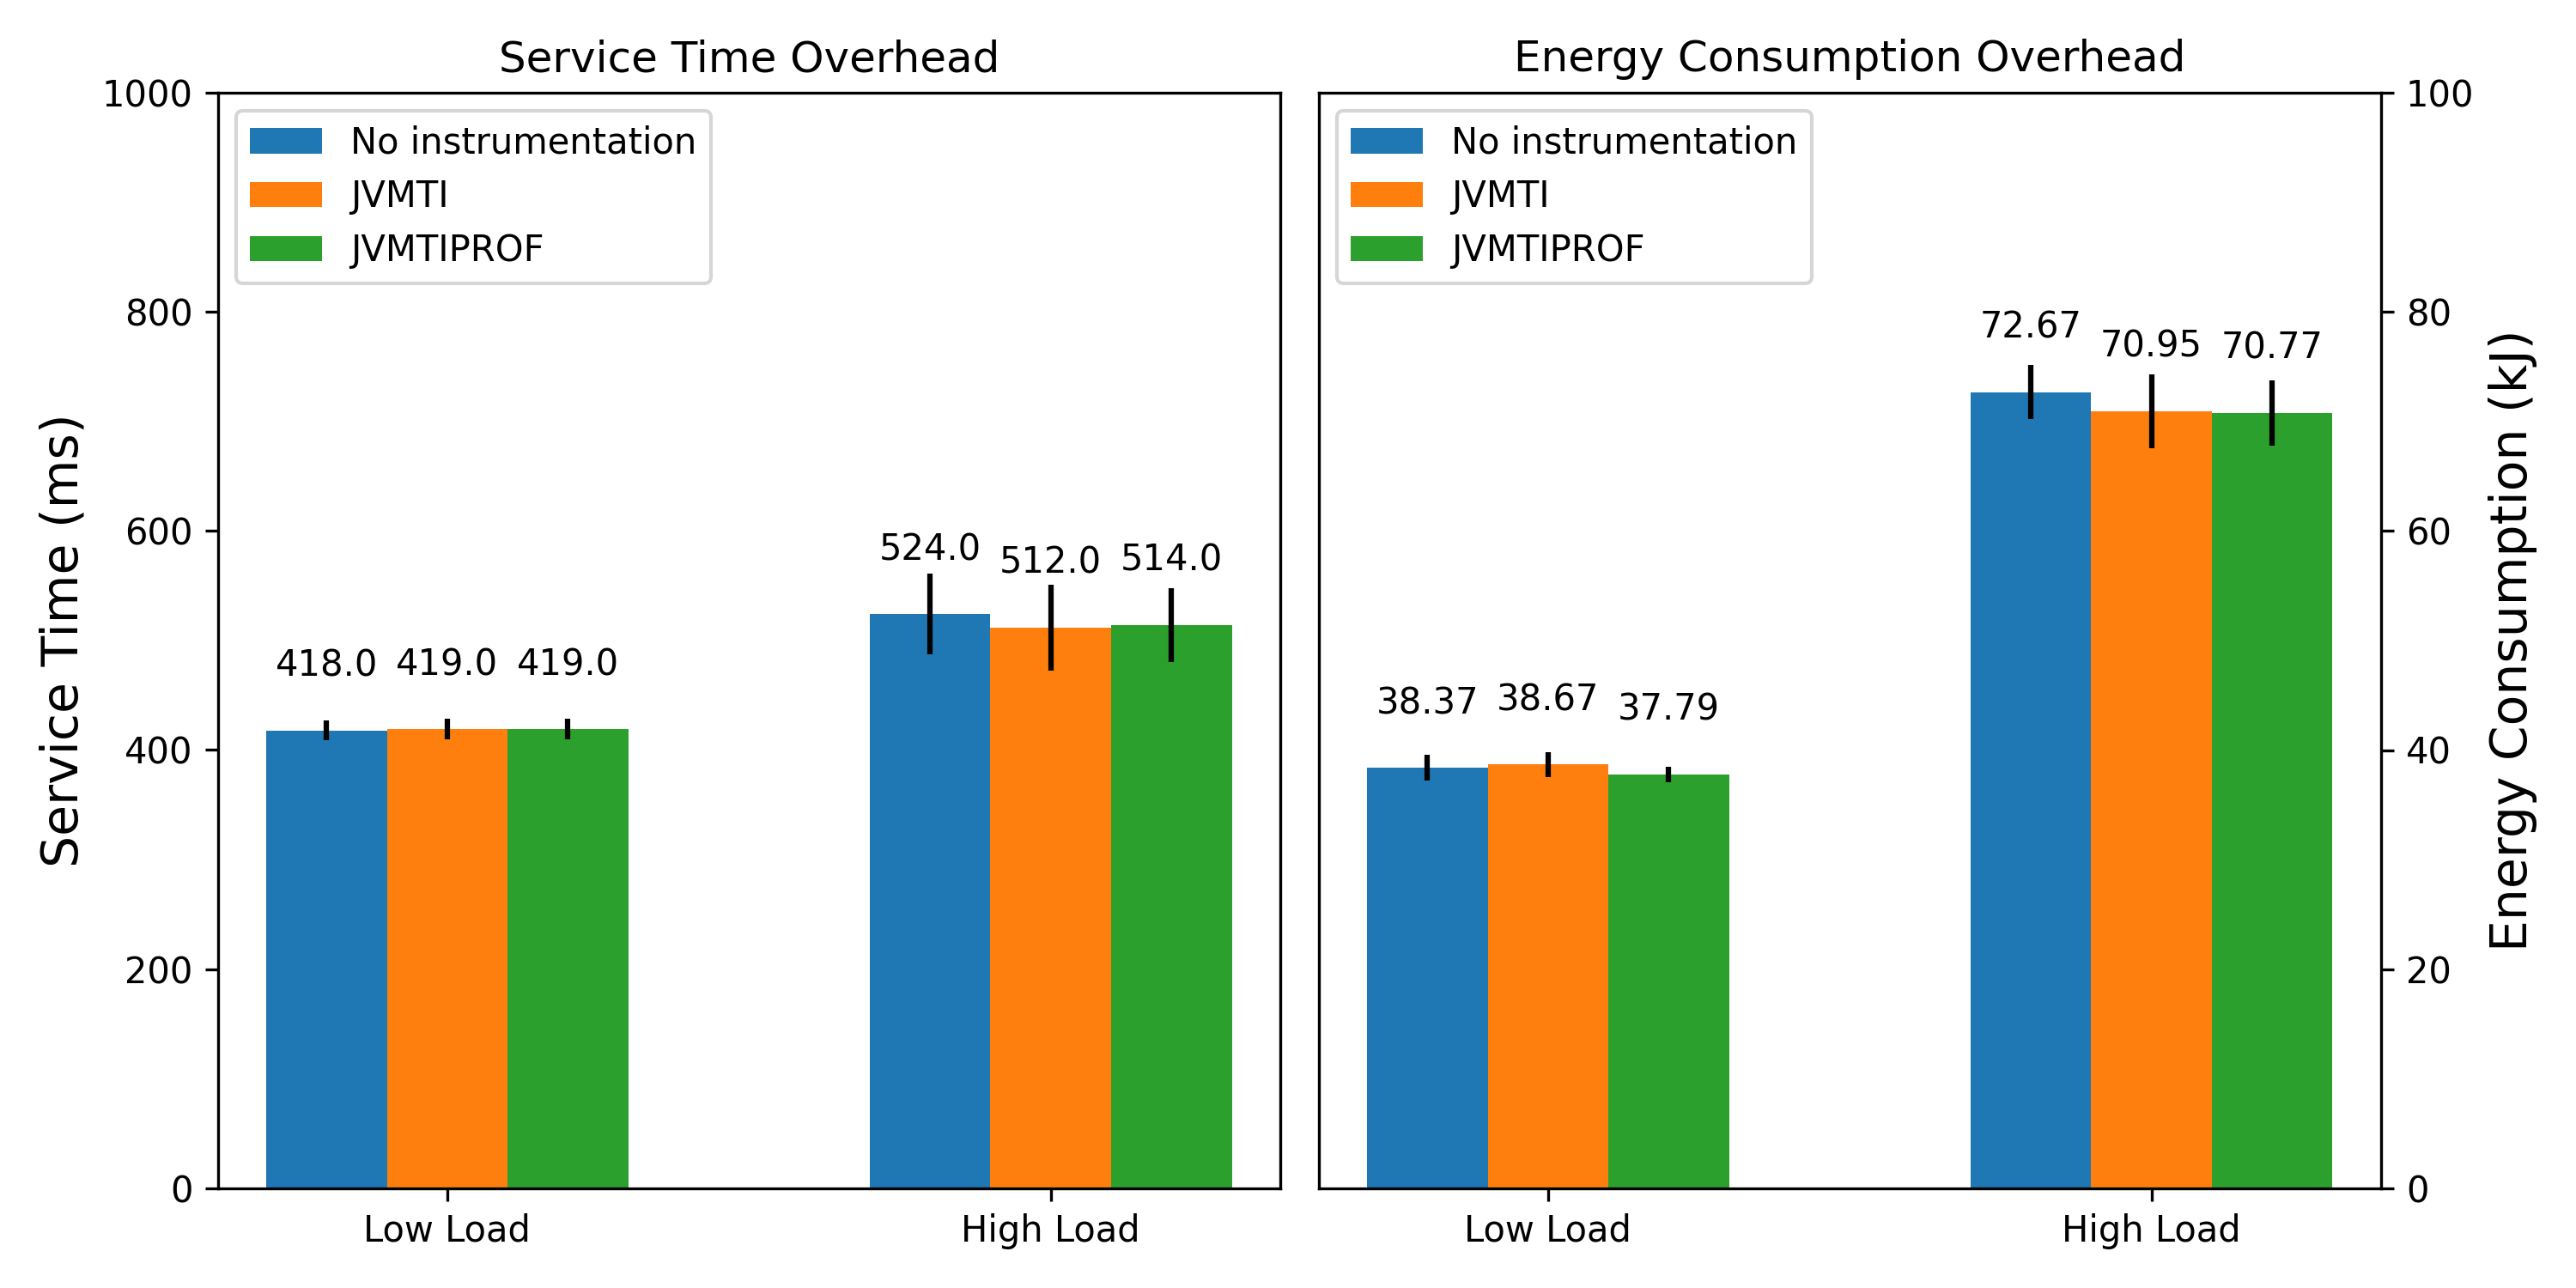
\includegraphics[width=1.0\textwidth]{src/figure/overhead.png}
\end{frame}

\section{Concluding Remarks}

\begin{frame}
\frametitle{Concluding Remarks}
\begin{itemize}
\item<1-> Minimal performance penalties compared to JVMTI.
\item<2-> Extending JVMTI
\begin{itemize}
\item ...by manipulating its function table is hard to maintain.
\item Alternative: JVMTI environment private to JVMTIPROF.
\end{itemize}
\item<3-> Future Work
\begin{itemize}
\item<3-> Cross-platform support.
\item<4-> Additional functionalities (e.g. capture arguments).
\item<5-> Hybrid call stack tracing (PANGIN, 2016).
\item<6-> Method interception by generating specialized code.
\item<7-> Execution sampling with a per-thread timer.
\end{itemize}
\end{itemize}
\end{frame}

\begin{frame}
\begin{center}
\usebeamerfont*{frametitle}
Thank You!
\end{center}
\end{frame}

\end{document}
